% Presentation on the 3x+1 Problem for Research Methods in Applied Maths
% 03.03.2020, Moritz Konarski, AUCA

%==============================================================================
% SETUP

\documentclass[hyperref={colorlinks,allcolors=black}]{beamer}

% this template is available at: 
% https://www.overleaf.com/latex/templates/beamer-presentation/jvmwtkmnqtpp

% set looks of the presentation
\mode<presentation>
{
  \usetheme{Goettingen}                     % set general look
  \usecolortheme{seahorse}                  % set color scheme
  \usefonttheme{serif}                      % set font to latex-like
  \setbeamertemplate{navigation symbols}{}
  \setbeamertemplate{caption}[numbered]
} 

% packages used
\usepackage[english]{babel}
\usepackage[utf8]{inputenc}
\usepackage[T1]{fontenc}
\usepackage{amsmath}
\usepackage{amsfonts}
\usepackage{textcomp}
\usepackage{graphicx}
\graphicspath{{../graphics/}}
\usepackage{epstopdf}

% create section title slides
\AtBeginSection[]{
    \begin{frame}
    \vfill
    \centering
    \begin{beamercolorbox}[sep=8pt,center,shadow=false,rounded=false]{title}
    \usebeamerfont{title}\insertsectionhead\par
    \end{beamercolorbox}
    \vfill
    \end{frame}
}

%==============================================================================
% PRESENTATION

%------------------------------------------------------------------------------
% GENERAL INFORMATION

\title[$3x+1$ Problem]{An Overview of the $3x+1$ Problem}
\author[M. Konarski]{Moritz M. Konarski}
\institute[AUCA]{Applied Mathematics Department \newline 
    American University of Central Asia}
\date{March 3rd, 2020}

\begin{document}

\begin{frame}
  \titlepage
\end{frame}

\begin{frame}{Outline}
  \tableofcontents
\end{frame}

%------------------------------------------------------------------------------
% INTRODUCTION

\section{Introduction}

\subsection[Function]{The $3x+1$ Function}

%------------------------------------------------------------------------------

\begin{frame}{The $3x+1$ Function}
The $3x+1$ Problem is based on the \textbf{Collatz Function}

\begin{equation}
\nonumber
C(x)= \left\{
    \begin{array}{ll}
        3x+1 \quad &\text{if } x \equiv 1 \text{ (mod 2),} \\
        x/2 \quad &\text{if } x \equiv 0 \text{ (mod 2).}
    \end{array}
\right.
\end{equation}

When the $3x+1$ Problem is studied, the \textbf{$3x+1$ Function}

\begin{equation}
\nonumber
T(x)= \left\{
    \begin{array}{ll}
        (3x+1)/2 \quad &\text{if } x \equiv 1 \text{ (mod 2),} \\
        x/2 \quad &\text{if } x \equiv 0 \text{ (mod 2).}
    \end{array}
\right.
\end{equation}

is used.
\end{frame}

%------------------------------------------------------------------------------

\begin{frame}{The $3x+1$ Function}
\begin{itemize}
    \item $T(x)$ is a function in \textbf{number theory}
    \item domain of $T(x)$ are positive integers, its range are positive 
        integers
    \item mathematically, 
        $T(x)$ maps $\mathbb{N} + 1 \rightarrow \mathbb{N} + 1$ 
    \item $T(x)$ has a \textbf{stopping time}, \textbf{total stopping 
        time}, and \textbf{trajectory} for each $x \in \mathbb{N} + 1$
    \item $T(x)$ is repeatedly applied to an initial $x$
\end{itemize}
\end{frame}

%------------------------------------------------------------------------------

\begin{frame}{Collatz Conjecture}
\begin{block}{Conjecture}
For all $x \in \mathbb{N} + 1$ there is a $k \in \mathbb{N} + 1$ such that
$T^{(k)}(x)=1$.
\end{block}

\begin{itemize}
    \item starting at any positive integer $x$, $k$ iterations of $T(x)$ will 
        give the result 1
    \item the Collatz Conjecture has \textbf{not been proven}
\end{itemize}
\end{frame}

%------------------------------------------------------------------------------

\begin{frame}{Possible Behavior of $T(x)$}
$T(x)$ can:
\begin{enumerate}
    \item reach 1, which is equivalent to entering the \textbf{trivial cycle} 
        $\{2,1,2,1,\dots\}$
    \item enter a non-trivial cycle that does not include 1
    \item diverge to infinity and not enter any type of cycle
\end{enumerate}
    The Collatz Conjecture states that \textbf{1. always happens}.
\end{frame}

%------------------------------------------------------------------------------

\subsection[Background]{Background Information}

\begin{frame}{Background Information}
\begin{itemize}
    \item named after German mathematician Lothar Collatz
    \item problem circulated since the 1950s
    \item academic publications started in the 1970s
    \item conjecture has been verified for over $10^{20}$ numbers
    \item most recent progress was in September of 2019
    \item problem is still being actively researched
\end{itemize}
\end{frame}

%------------------------------------------------------------------------------

\begin{frame}{Reasons to Study the Problem}
\begin{itemize}
    \item problem is simple to state, but hard to prove
    \item remains unsolved after over 50 years of research
    \item iterative mappings are currently a popular research topic
    \item verifying large numbers is computationally interesting
    \item could yield results connected to prime factorization using 2 and 3
\end{itemize}
\begin{quote}
Mathematics is not ready for such problems. \\ \flushright --- Paul Erdös
\end{quote}
\end{frame}

%------------------------------------------------------------------------------
% DETAILS

\section[Details]{$3x+1$ Problem in Detail}

\subsection{Trajectories}

%------------------------------------------------------------------------------

\begin{frame}{Trajectory}
\begin{itemize}
    \item the trajectory of $x$ under $T(x)$ is the set of successive
        iterations of $T(x)$
    \item it is also called the forward orbit $O^+(x)$ of $x$ under $T(x)$
    \item trajectories can be graphed 
\end{itemize}
\begin{equation}
    \nonumber
    O^+(x):=\{x, T(x), T^{(2)}(x), T^{(3)}(x),\dots\}
\end{equation}
\end{frame}

%------------------------------------------------------------------------------

\begin{frame}{Example: Trajectory of $T(39)$}
The trajectory of $T(39)$ is
\begin{align}
    \nonumber
    O^+(39):=\{&39,59,89,134,67,101,152,76,38,19,29,\\
    \nonumber
               &44,22,11,17,26,13,20,10,5,8,4,2,1\}
\end{align}
and can be graphed like this for $k$ and $T^{(k)}(39)$
\begin{figure}
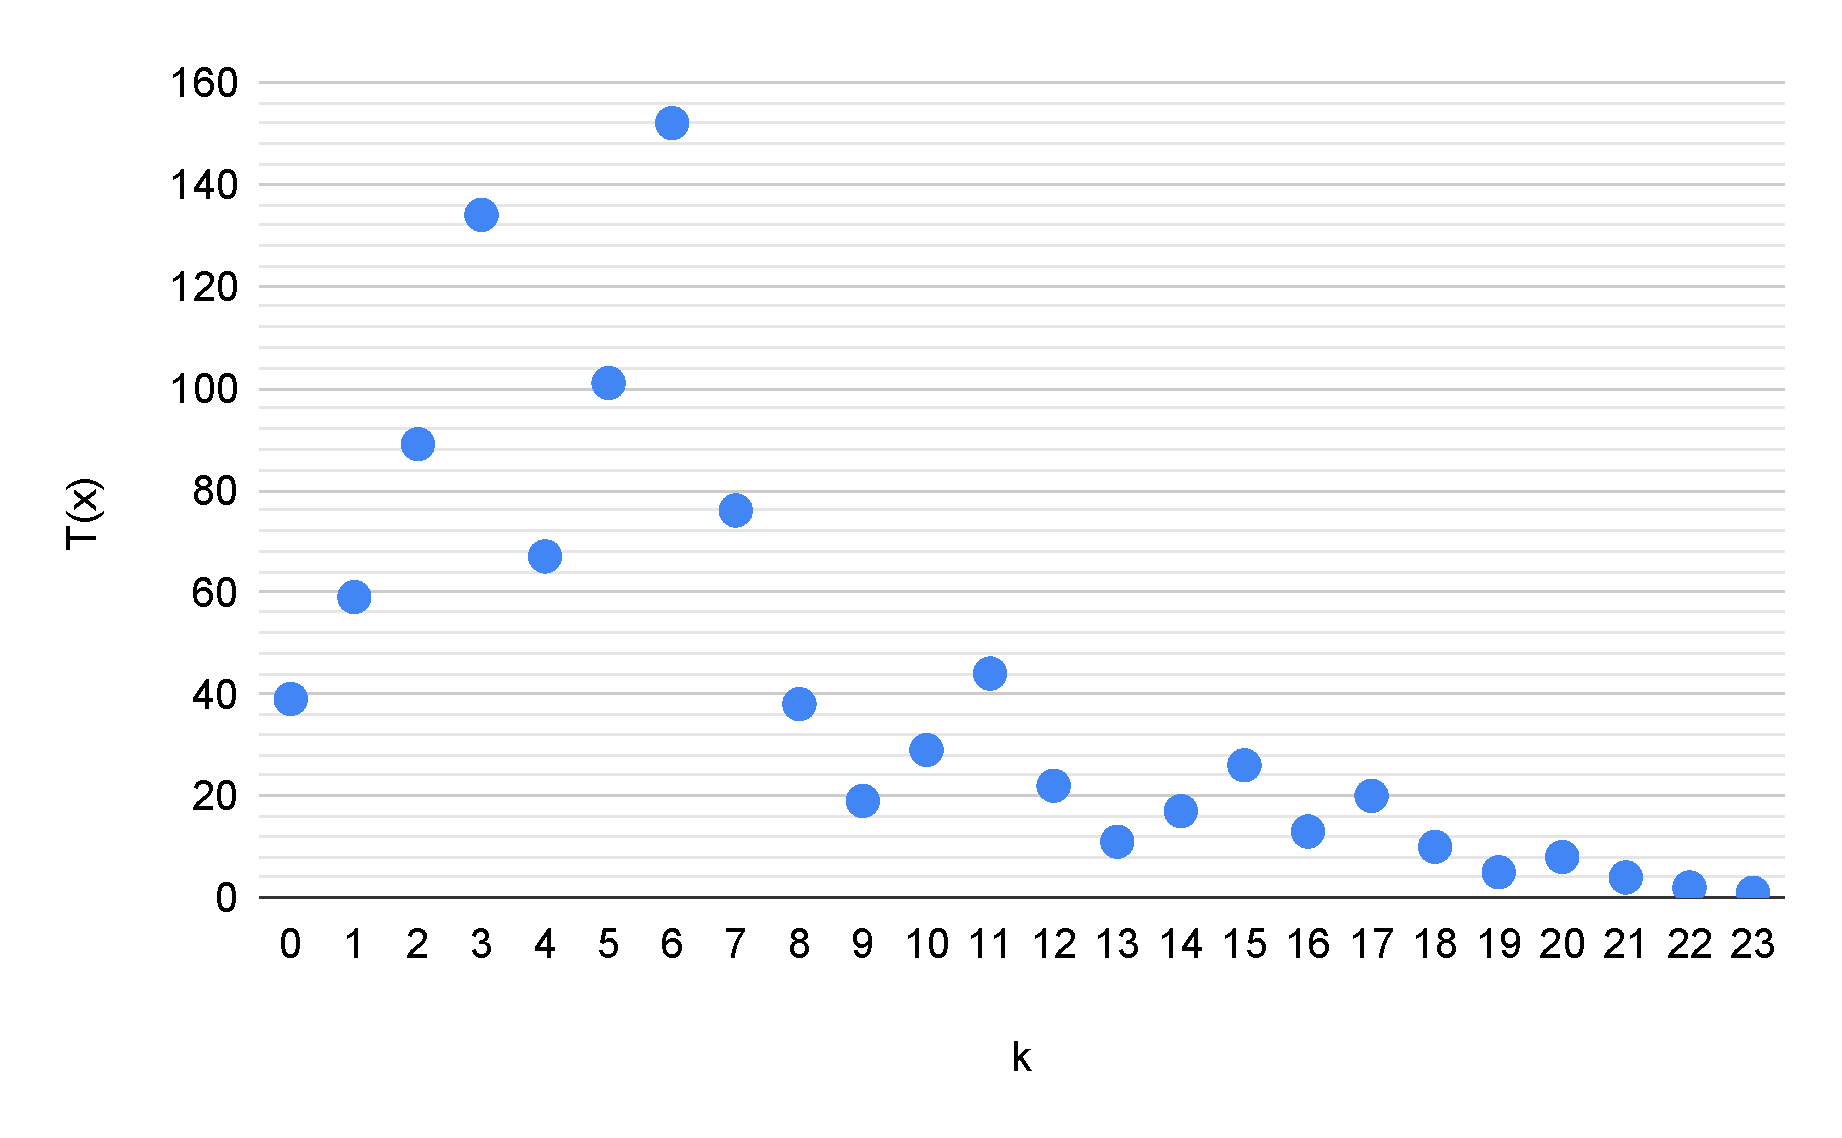
\includegraphics[scale=0.3]{trajectory_graph.pdf}
\end{figure}
\end{frame}

%------------------------------------------------------------------------------

\subsection{Cycles}

%------------------------------------------------------------------------------

\begin{frame}{Cycles}
\begin{itemize}
    \item $T(x)$ has the \textbf{trivial cycle} $\{2,1,2,\dots\}$, which is
        equivalent to reaching 1
    \item the Collatz Conjecture states that \textbf{all orbits will 
        eventually enter the trivial cycle} and thus that \textbf{it is the 
        only cycle}
    \item if $T(x)$ has non-trivial cycles, they have been proven to be over
        10.4 billion numbers long
\end{itemize}
\end{frame}

%------------------------------------------------------------------------------

\subsection{Stopping Time}

%------------------------------------------------------------------------------

\begin{frame}{Stopping Time}
\begin{itemize}
    \item the number of iterations of $T(x)$ until the result is smaller
        than $x$
    \item first it is checked that every positive integer up to $x - 1$ 
        iterates to 1
    \item then, if $T^{(k)}(x) < x$, we know it will iterate to 1
    \item if the Collatz Conjecture is true, all $x \in \mathbb{N} + 1$ have
        a finite stopping time
\end{itemize}
\begin{equation}
    \nonumber
    \sigma(x)=\inf\{k:T^{(k)}(x) < x\}
\end{equation}
\end{frame}

%------------------------------------------------------------------------------

\begin{frame}{Example: Stopping time of $T(39)$}
With the trajectory of $T(39)$
\begin{align}
    \nonumber
    O^+(39):=\{&39,59,89,134,67,101,152,76,\textbf{38},19,29,\\
    \nonumber
               &44,22,11,17,26,13,20,10,5,8,4,2,1\},
\end{align}
we see that 38 is the first number <39. \\Thus $\sigma(39) = 8$, as 38
is the result of the 8th iteration.
\end{frame}

%------------------------------------------------------------------------------

\begin{frame}{Total Stopping Time}
The total stopping time is the number of steps needed for $T(x)$ to iterate to 
1. It is defined as
\begin{equation}
    \nonumber
    \sigma_{\infty}(x)=\inf\{k:T^{(k)}(x)=1\} 
\end{equation}
\begin{block}{Example for $\sigma_{\infty}(39)$}
For $T(39)$,
\begin{align}
    \nonumber
    O^+(39):=\{&39,59,89,134,67,101,152,76,38,19,29,\\
    \nonumber
               &44,22,11,17,26,13,20,10,5,8,4,2,1\}
\end{align}
and we see that $T^{(23)}(39)=1$, so $\sigma_{\infty}(39)=23$.
\end{block}
\end{frame}

%------------------------------------------------------------------------------

\subsection[Approximations]{Stochastic Approximations}

\begin{frame}{Stochastic Approximations}
\begin{itemize}
    \item each trajectory has approximately the same number of odd and even 
        elements
    \item the behavior of $T(x)$ is pseudorandom for large numbers
    \item thus, probabilistic models describe its behavior
    \item these models describe groups of trajectories
    \item e.g., the upper bound for $\sigma_{\infty}$ is $41.677647 \log x$
\end{itemize}
\end{frame}

%------------------------------------------------------------------------------

\begin{frame}{Example: Stopping Time Approximations}
The total stopping time for most trajectories is approximated to be about 
$6.95212 \log x$ steps.
\begin{block}{Example for $T(39)$}
For $T(39)$ we have the approximation
\begin{equation}\nonumber
    6.95212 \log 39 \approx 25.4952
\end{equation}
Compared to the known $\sigma_{\infty}(39)=23$ this is not bad.
\end{block}
\end{frame}

%------------------------------------------------------------------------------
% SUMMARY

\section{Summary}

\begin{frame}{Summary}
\begin{itemize}
    \item the Collatz Conjecture states that for $x,k \in \mathbb{N} + 1$
        $T^{(k)}(x)=1$
    \item the conjecture has not been proven, but verified for $10^{20}$
        numbers
    \item all orbits of $T(x)$ should reach the trivial cycle
    \item $T(x)$ can be probabilistically described because of pseudo-randomness
\end{itemize}
\end{frame}


%==============================================================================
% BIBLIOGRAPHY

\begin{frame}{References}
\begin{thebibliography}{4}

\bibitem{chamberland} Marc Chamberland, 
    \textit{An Update on the $3x+1$ Problem},
        \texttt{http://www.math.grinnell.edu/\~{}chamberl/papers\\
        /3x\_survey\_eng.pdf},
    2005.

\bibitem{crandall} R. E. Crandall, \textit{On the "$3x+1$" Problem},
    Mathematics of Computation, \textbf{32} (1978), no. 144, 1281-1292.

\bibitem{lagarias} Jeffrey C.Lagarias, 
    \textit{The $3x+1$ Problem: An Overview},
    \texttt{https://pdfs.semanticscholar.org/100046dd8b4ee\\
        901bc71043da7d42f5d87ca0224.pdf},
    2010.

\bibitem{tao} Terence Tao, \textit{Almost All Orbits of the Collatz Map Attain
    Almost Bounded Values}, arXiv:1909.03562v2 [math.PR], 2019.

\end{thebibliography}
\end{frame}
\end{document}

\end{document}
